% !TEX root = holder_flie.tex

\chapter{\chap{Monte Carlo Method}}
%%

%----------  section ------------
\section{Monte Carlo Method}
\noindent The Monte Carlo Simulation, which uses a large number of random numbers, may prove to be a better alternative when there is a high level of uncertainty for estimating or predicting, as opposed to just replacing the uncertain variable with a single average number.\\[2mm]
For processes that are difficult to forecast because of the involvement of random variables, Monte Carlo methods are used to model the likelihood of various outcomes. It is a method for comprehending how risk and uncertainty affect forecasting and prediction models.
\section{Monte Carlo Simulation History}
Since chance and random results are essential to the modeling technique, just as they are to games like roulette, dice, and slot machines, Monte Carlo simulations are called after the well-known gambling location in Monaco.
Stanislaw Ulam, a mathematician who worked on the Manhattan Project, invented the method initially. Ulam kept himself occupied after the war while he recovered from brain surgery by playing endless rounds of solitaire. He developed an interest in graphing the results of each of these games so that he could examine their distribution and calculate the likelihood of winning. John Von Neumann and he worked together to create the Monte Carlo simulation after sharing their concept.
\section{History of Monte Carlo in Finance}
David B. Hertz published an essay in the Harvard Business Review in 1964 outlining the use of Monte Carlo methods in corporate finance, which was the first to bring them to the attention of the finance industry. Phelim Boyle was the first to employ simulation in the valuation of derivatives in his key Journal of Financial Economics work from 1977.\\[2mm]

%%\ref{https://www.youtube.com/channel/UCUcpVoi5KkJmnE3bvEhHR0Q}


\section{A Practical Example with Code}
\noindent Dart problem is a nice illustration for best comprehending the Monte Carlo approach. In this issue, we'll assume that there is a square with side 2 units, and that there is a circle with radius 1 units inside the square. Now that we know the probability of striking the circle if we toss a dart into the square, we must throw the dart at random.\\[2mm]

Therefore, on a 2-D plane with a domain defined as a square with a side of 2 units and centered on (0,0). Imagine a circle with the same radius as the square—one unit—within the same domain. The ratio between the number of points inside the circle and the overall number of points generated is then determined. \\
the area of that circle is $C=\pi$ \\
the area of that square is $S=4$ \\
the ratio would be
$\frac{C}{S}=\frac{\pi}{4}=\frac{\text{no. of points in }C}{\text{no. of points in }S}$\\[2mm]

we have to generate some random numbers for (x, y) then test it if it satisfies the following inequality 
$$x^2+y^2<=1$$. 


However, the frequency interpretation of probability informs us that as the number of trials rises, the approximation becomes more precise. Let's increase the number of trials and plot the results to see why this is the case. I ran simulations between 100 and 1000 times. Below is a display of the simulations' outcomes.\\

\subsection{Convergence of Monte Carlo}
\begin{figure}[H]
	\begin{center}
		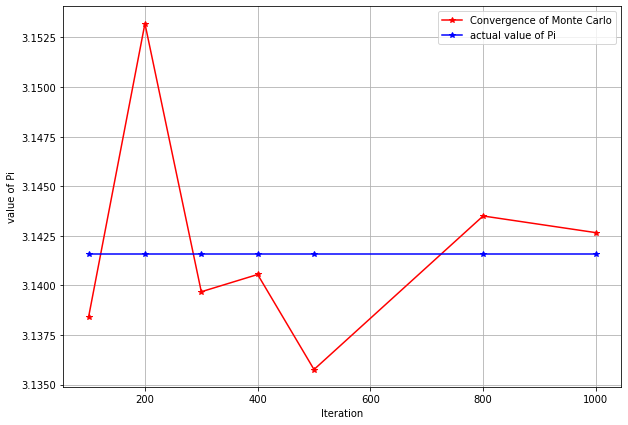
\includegraphics[width=0.8\textwidth]{dart_prob}
	\end{center}
	\caption{Convergence of Monte Carlo}
\end{figure}

\noindent From this graph we can say that MC method can converge to its actual value if we increase the number of iteration. 

\begin{table}[H]
	\begin{center}
		\begin{NiceTabular}{|c|c|c|}[hvlines]
			\rowcolor{blue!20} Serial No. & Interval & Output  \\ 
			1 & 100 & 3.1384 \\
			2 & 200 & 3.1532 \\
			3 & 300 & 3.13968 \\
			4 & 400 & 3.14055 \\
			5 & 500 & 3.13576  \\ 
			6 & 800 & 3.1435  \\ 
			7 & 1000 & 3.14266  \\
			
		\end{NiceTabular}
	\end{center}
	\caption{Monte Carlo Method for Dart Problem}
\end{table}
%\url{https://colab.research.google.com/drive/1VQ95AiamlMWGvvWfpMmaV1nH_NNBiNgG?usp=sharing}


